% 三矢量的混合积
% 线性代数|矢量|叉乘|内积|混合积|行列式

\pentry{矢量的叉乘\upref{Cross}}
我们定义以下运算
\begin{equation}
(\bvec A \cross \bvec B) \vdot \bvec C
\end{equation}
为矢量 $\bvec A, \bvec B, \bvec C$ 的\textbf{混合积}. 混合积满足
\begin{equation}\label{TriVM_eq1}
(\bvec A \cross \bvec B) \vdot \bvec C = (\bvec B \cross \bvec C) \vdot \bvec A = (\bvec C \cross \bvec A) \vdot \bvec B 
\end{equation} 
这个公式可由\autoref{TriVM_fig1} 记忆.
\begin{figure}[ht]
\centering % 未完成: 把这个图改成圆圈, 每个箭头变成弧线. 要不然会误以为箭头代表矢量. 另外就是搞两张图, 一张顺时针一张逆时针
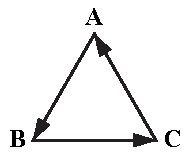
\includegraphics[width=3.2cm]{./figures/TriVM_1.pdf}
\caption{\autoref{TriVM_eq1} 记忆法}\label{TriVM_fig1}
\end{figure}
图中箭头的方向由叉乘的方向(顺时针或逆时针)决定,与内积无关, 即 $\bvec A\cross \bvec B \vdot \bvec C = \bvec C \vdot (\bvec A \cross \bvec B)$.如果混合积的顺序取与箭头相反的方向, 根据叉乘的性质,需要在前面加上负号(叉乘不满足乘法交换律). \autoref{TriVM_eq1} 与\autoref{TriVM_eq2} 互为相反数
\begin{equation}\label{TriVM_eq2}
(\bvec C \cross \bvec B) \vdot \bvec A = (\bvec B \cross \bvec A) \vdot \bvec C = (\bvec A \cross \bvec C) \vdot \bvec B
\end{equation}

注意即使将混合积省略括号记为 $\bvec A \cross \bvec B \vdot \bvec C$ 或者 $\bvec C \vdot \bvec A \cross \bvec B$ 也应该理解为先叉乘后内积. $\bvec A \cross (\bvec B \vdot \bvec C)$ 没有定义, 因为矢量不能叉乘标量.

\subsection{几何法证明}

\begin{figure}[ht]
\centering
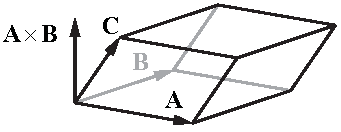
\includegraphics[width=6cm]{./figures/TriVM_2.pdf}
\caption{矢量混合积的几何意义} \label{TriVM_fig2}
\end{figure}

如\autoref{TriVM_fig2}, 以三个矢量为棱作平行六面体. 由\autoref{Cross_exe1}~\upref{Cross} 可知 $\abs{\bvec A \cross \bvec B}$ 就是 $\bvec A,\bvec B$ 所在平行四边形的面积. 令 $\bvec A \cross \bvec B = \abs{\bvec A \cross \bvec B} \uvec n$, 则 $\uvec n$ 为平面的法向量, 平行六面体的高为 $\abs{\uvec n \vdot \bvec C}$, 所以平行六面体的体积等于底面积乘以高
\begin{equation}
V = \abs{\bvec A \cross \bvec B} \abs{\uvec n \vdot \bvec C} = \abs{\bvec A \cross \bvec B \vdot \bvec C}
\end{equation}
同理可得对于同一平行六面体
\begin{equation}
V = \abs{\bvec B \cross \bvec C \vdot \bvec A} = \abs{\bvec C \cross \bvec A \vdot \bvec B} 
\end{equation}  
这里只证明了\autoref{TriVM_eq1} 的绝对值, 要证明正负号, 定义 $\uvec n \vdot \bvec C < 0$ 时 $V$ 为负值即可.

\subsection{代数法证明}
\pentry{行列式\upref{Deter}}
不难证明三矢矢积若展开成分量的形式,等于三个矢量组成的行列式
\begin{equation}
\bvec A \cross \bvec B \vdot \bvec C = \vmat{
A_x & A_y & A_z\\
B_x & B_y & B_z\\
C_x & C_y & C_z}
\end{equation}
而利用行列式中任意两行置换符号改变,即可证明\autoref{TriVM_eq1}.
